
\begin{figure}[ht!]
\centering
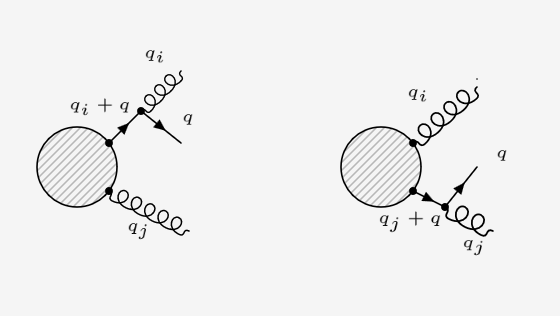
\includegraphics[width=0.85\textwidth]{images/GQ/GQDiagrams.png}
\end{figure}

\pagebreak

\section{$ M_1 $}
\begin{figure}[ht!]
\centering
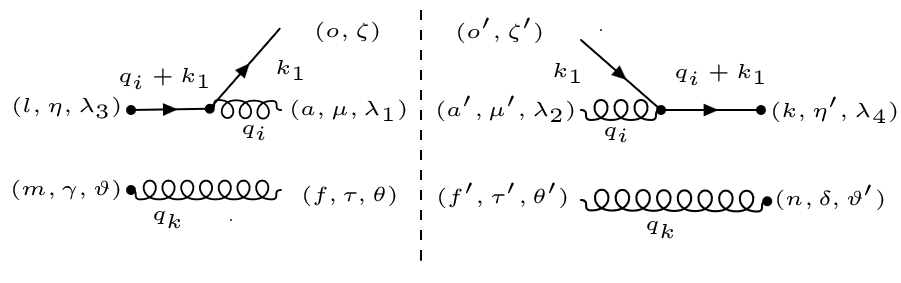
\includegraphics[scale=0.7]{images/GQ/M1Squer.png}
\end{figure}

\begin{equation}
\begin{split}
|M_1|^2=-\frac{{g_s}^2 {[T^{a^{\prime}}]_k}^{o^{\prime}} {[T^a]_{o}}^{l}}{4(k_1 \cdot q_i)(k_1 \cdot q_i)}[\not{k_1}{\gamma}^{\mu}(\not{q_i}+\not{k_1})\:\:(\not{q_i}+\not{k_1}) {\gamma}_{{\mu}}][-{g^{\delta}}_{\gamma}]
\end{split}
\end{equation}

\begin{equation}
\begin{split}
|M_1|^2=-\frac{{g_s}^2 {[T^{a^{\prime}}]_k}^{o^{\prime}} {[T^a]_{o}}^{l}}{4(k_1 \cdot q_i)(k_1 \cdot q_i)}[\not{k_1}{\gamma}^{\mu}(\not{q_i}\not{k_1}+\not{k_1}\not{q_i}) {\gamma}_{{\mu}}][-{g^{\delta}}_{\gamma}]
\end{split}
\end{equation}

\begin{equation}
\begin{split}
|M_1|^2=-\frac{{g_s}^2 {[T^{a^{\prime}}]_k}^{o^{\prime}} {[T^a]_{o}}^{l}}{4(k_1 \cdot q_i)(k_1 \cdot q_i)}
[\not{k_1}{\gamma}^{\mu}\not{q_i}\not{k_1}{\gamma}_{{\mu}}+\not{k_1}{\gamma}^{\mu}\not{k_1}\not{q_i} {\gamma}_{{\mu}}][-{g^{\delta}}_{\gamma}]
\end{split}
\end{equation}

\begin{equation}
\begin{split}
|M_1|^2=-\frac{{g_s}^2 {[T^{a^{\prime}}]_k}^{o^{\prime}} {[T^a]_{o}}^{l}}{4(k_1 \cdot q_i)(k_1 \cdot q_i)}
[\not{k_1}{\gamma}^{\mu}(2q_i \cdot k_1 -\not{k_1}\not{q_i}){\gamma}_{{\mu}}+\not{k_1}{\gamma}^{\mu}\not{k_1}\not{q_i} {\gamma}_{{\mu}}][-{g^{\delta}}_{\gamma}]
\end{split}
\end{equation}

\begin{equation}
\begin{split}
|M_1|^2=-d\frac{{g_s}^2 C_F}{2(k_1 \cdot q_i)}
[\not{k_1}][-{g^{\delta}}_{\gamma}]
\end{split}
\end{equation}

\begin{equation}
\begin{split}
|M_1|^2=-d\frac{{g_s}^2 C_F}{2y\:p_i \cdot Q}
[(\alpha_1 -y\beta_1(\frac{Q^2}{2p_i \cdot Q})) \not{p_i} + y\beta_1\not{Q} + \sqrt{y\alpha_1\beta_1}\not{n}_{\bot,1}][-{g^{\delta}}_{\gamma}]
\end{split}
\end{equation}

\begin{equation}
\begin{split}
|M_1|^2=-d(1-\beta_1)\frac{{g_s}^2 C_F}{2y \:p_i \cdot Q}
[  \not{p_i}][-{g^{\delta}}_{\gamma}]
\end{split}
\end{equation}

\pagebreak

\section{$ M_2 $}
\begin{figure}[ht!]
\centering
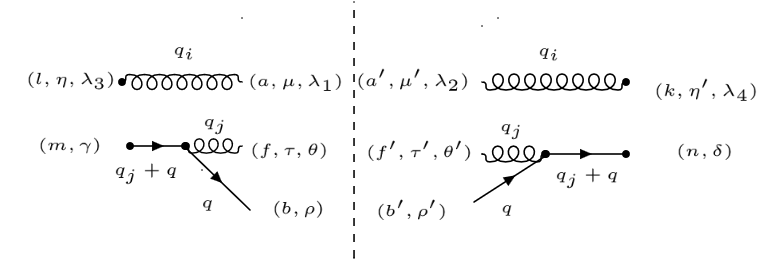
\includegraphics[scale=0.7]{images/GQ/M2Squer.png}
\end{figure}

\begin{equation}
\begin{split}
|M_2|^2=-\frac{{g_s}^2 C_F}{4(k_1 \cdot q_k)(k_1 \cdot q_k)}[\not{k_1}{\gamma}^{\tau}(\not{q_k}+\not{k_1})\:\:(\not{q_k}+\not{k_1}) {\gamma}_{{\tau}^{\prime}}][-g^{{\eta}{\eta}^{\prime}}]
\end{split}
\end{equation}

\begin{equation}
\begin{split}
|M_2|^2=-\frac{{g_s}^2 C_F}{4(k_1 \cdot q_k)(k_1 \cdot q_k)}[\not{k_1}{\gamma}^{\tau}(\not{q_k}\not{k_1}+\not{k_1}\not{q_k}) {\gamma}_{{\tau}^{\prime}}][-g^{{\eta}{\eta}^{\prime}}]
\end{split}
\end{equation}

\begin{equation}
\begin{split}
|M_2|^2=-\frac{{g_s}^2 C_F}{4(k_1 \cdot q_k)(k_1 \cdot q_k)}
[\not{k_1}{\gamma}^{\mu}\not{q_k}\not{k_1}{\gamma}_{{\tau}}+\not{k_1}{\gamma}^{\mu}\not{k_1}\not{q_k} {\gamma}_{{\tau}^{\prime}}][-g^{{\eta}{\eta}^{\prime}}]
\end{split}
\end{equation}

\begin{equation}
\begin{split}
|M_2|^2=-\frac{{g_s}^2 C_F}{2(k_1 \cdot q_k)}
[\not{k_1}][-g^{{\eta}{\eta}^{\prime}}]
\end{split}
\end{equation}

\begin{equation}
\begin{split}
|M_2|^2=-\frac{{g_s}^2 C_F}{2(1-\beta_1) (1-y)\:p_i \cdot p_k}
[(\alpha_1 -y\beta_1(\frac{Q^2}{2p_i \cdot Q})) \not{p_i} + y\beta_1\not{Q} + \sqrt{y\alpha_1\beta_1}\not{n}_{\bot,1}][-g^{{\eta}{\eta}^{\prime}}]
\end{split}
\end{equation}

\begin{equation}
\begin{split}
|M_2|^2=-d\frac{{g_s}^2 C_F}{2 (1-y)\:p_i \cdot p_k}
[ \not{p_i}][-g^{{\eta}{\eta}^{\prime}}]
\end{split}
\end{equation}

It doesn't contribute to the final result!!

\pagebreak

\section{$ M1{M_2}^{\dagger} $}

\begin{figure}[ht!]
\centering
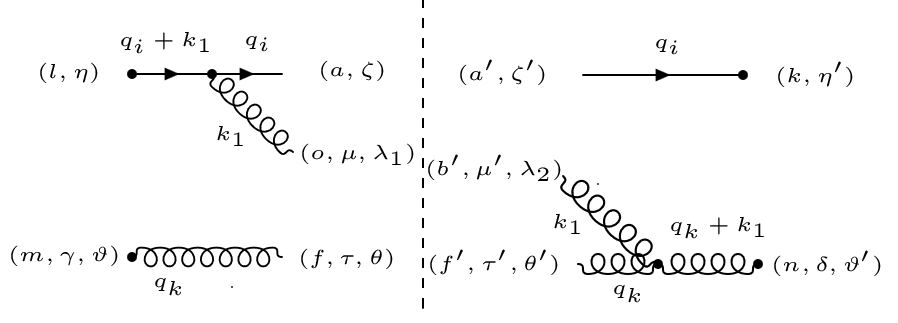
\includegraphics[scale=0.7]{images/GQ/M1M2DaggerGluon.png}
\end{figure}

\begin{equation}
\begin{split}
&M1{M_2}^{\dagger}=\frac{-{g_s}^2 {[T^{o}]_a}^{l} f^{\:f^{\prime}\: b^{\prime}\:n}}{4(k_1 \cdot q_i)(k_1 \cdot q_k)}[\not{q_i}{\gamma}_{\mu}(\not{k_1}+\not{q_i})\:]\\
&[ (g^{{{\gamma}}{{\mu}}}(q_k-k_1)^{\delta}+g^{{{\mu}}{{\delta}}}(2k_1 +q_k)^{{\gamma}}-g^{\delta{{\gamma}}}(2q_k+k_1)^{{\mu}})]\\
\end{split}
\end{equation}

\begin{equation}
\begin{split}
&M1{M_2}^{\dagger}=\frac{-{g_s}^2 {[T^{o}]_a}^{l} f^{\:f^{\prime}\: b^{\prime}\:n}}{4(k_1 \cdot q_i)(k_1 \cdot q_k)}[-\gamma_{\mu}\not{q_i}\not{k_1+2}(\not{k_1}+\not{q_i}){q_i}_{\mu}\:]\\
&[ g^{{{\gamma}}{{\mu}}}(q_k-k_1)^{\delta}+g^{{{\mu}}{{\delta}}}(2k_1+q_k )^{{\gamma}}-g^{\delta{{\gamma}}}(2q_k+k_1)^{{\mu}}]\\
\end{split}
\end{equation}

\begin{equation}
\begin{split}
&M1{M_2}^{\dagger}=\frac{-{g_s}^2 {[T^{o}]_a}^{l} f^{\:f^{\prime}\: b^{\prime}\:n}}{4 y(1-\beta_1) (1-y)\:(p_i \cdot p_k)(p_i \cdot Q)}\\
&[-\gamma_{\mu}((\beta_1 -\alpha_1 y(\frac{Q^2}{2p_i \cdot Q}))\not{p_i} + y\alpha_1\not{Q})((\alpha_1 -y\beta_1(\frac{Q^2}{2p_i \cdot Q})) \not{p_i} + y\beta_1\not{Q})\\
&+(2((\alpha_1 -y\beta_1(\frac{Q^2}{2p_i \cdot Q})) \not{p_i} + 2y\beta_1\not{Q}+2(\beta_1 -\alpha_1 y(\frac{Q^2}{2p_i \cdot Q}))\not{p_i} + 2y\alpha_1\not{Q})(\beta_1{q_i}_{\mu})\:]\\
&[ g^{{{\gamma}}{{\mu}}}(-\alpha_1p_i)^{\delta}+g^{{{\mu}}{{\delta}}}(2\alpha_1p_i )^{{\gamma}}-g^{\delta{{\gamma}}}(\alpha_1p_i+(2-y)Q)^{{\mu}}]\\
\end{split}
\end{equation}

\begin{equation}
\begin{split}
&M1{M_2}^{\dagger}=\frac{-{g_s}^2 C_F}{4 y(1-\beta_1) (1-y)\:(p_i \cdot p_k)(p_i \cdot Q)}\\
&[-\gamma_{\mu}(y\beta_1^2)\not{p_i}\not{Q}+2(\not{p_i}+y\not{Q})(\beta_1{p_i}_{\mu})\:]\\
&[ g^{{{\gamma}}{{\mu}}}(-\alpha_1p_i+\sqrt{1-y} p_k)^{\delta}+g^{{{\mu}}{{\delta}}}(2\alpha_1p_i+ \sqrt{1-y} p_k)^{{\gamma}}-g^{\delta{{\gamma}}}(\alpha_1p_i+2\sqrt{1-y} p_k)^{{\mu}}]\\
\end{split}
\end{equation}

\begin{equation}
\begin{split}
&M1{M_2}^{\dagger}=\frac{-{g_s}^2 C_F}{4 y(1-\beta_1) (1-y)\:(p_i \cdot p_k)(p_i \cdot Q)}\\
&[-\gamma_{\mu}(y\beta_1^2)\not{p_i}\not{Q}][ g^{{{\gamma}}{{\mu}}}(-\alpha_1p_i+\sqrt{1-y} p_k)^{\delta}+g^{{{\mu}}{{\delta}}}(2\alpha_1p_i+ \sqrt{1-y} p_k)^{{\gamma}}-g^{\delta{{\gamma}}}(\alpha_1p_i+2\sqrt{1-y} p_k)^{{\mu}}]\\
&+[2(\not{p_i}+y\not{Q})(\beta_1{p_i}_{\mu})\:][ g^{{{\gamma}}{{\mu}}}(-\alpha_1p_i+\sqrt{1-y} p_k)^{\delta}+g^{{{\mu}}{{\delta}}}(2\alpha_1p_i+ \sqrt{1-y} p_k)^{{\gamma}}-g^{\delta{{\gamma}}}(\alpha_1p_i+2\sqrt{1-y} p_k)^{{\mu}}]\\
\end{split}
\end{equation}

\begin{equation}
\begin{split}
&M1{M_2}^{\dagger}=\frac{-{g_s}^2 C_F}{4 y(1-\beta_1) (1-y)\:(p_i \cdot p_k)(p_i \cdot Q)}\\
&[-\gamma_{\mu}(y\beta_1^2)\not{p_i}\not{Q}][ g^{{{\gamma}}{{\mu}}}(-\alpha_1p_i)^{\delta}+g^{{{\mu}}{{\delta}}}(\alpha_1p_i )^{{\gamma}}-g^{\delta{{\gamma}}}((2-y)Q)^{{\mu}}][{g^{\delta}}_{\gamma}]\\
&+[2\beta_1(\not{p_i}+y\not{Q})\:][{p_i}^{\gamma} (-\alpha_1p_i)^{\delta}+{p_i}^{\delta}(2\alpha_1p_i )^{{\gamma}}-g^{\delta{{\gamma}}}(\alpha_1p_i+(2-y))Q\cdot p_i]\\
\end{split}
\end{equation}

\begin{equation}
\begin{split}
&M1{M_2}^{\dagger}=\frac{-{g_s}^2 C_F}{4 y(1-\beta_1) (1-y)\:(p_i \cdot p_k)(p_i \cdot Q)}\\
&[-\gamma_{\mu}(y\beta_1^2)\not{p_i}\not{Q}][-g^{\delta{{\gamma}}}(\alpha_1p_i+2\sqrt{1-y} p_k)^{{\mu}}]\\
&+[2\beta_1(\not{p_i}+y\not{Q})\:][-g^{\delta{{\gamma}}}(\alpha_1p_i+2\sqrt{1-y})p_i\cdot p_k]\\
\end{split}
\end{equation}

\begin{equation}
\begin{split}
&M1{M_2}^{\dagger}=\frac{-{g_s}^2 C_F}{4 y(1-\beta_1) (1-y)\:(p_i \cdot p_k)(p_i \cdot Q)}\\
&[-2y\beta_1^2\sqrt{1-y} \not{p_k}\not{p_i}\not{Q}+4\sqrt{1-y}\beta_1(\not{p_i}+y\not{Q})p_i\cdot p_k][-g^{\delta{{\gamma}}}]\\
\end{split}
\end{equation}

\begin{equation}
\begin{split}
&M1{M_2}^{\dagger}=\frac{-{g_s}^2 C_F}{y(1-\beta_1) (1-y)\:(p_i \cdot Q)}\sqrt{1-y}\beta_1[\not{p_i}][-g^{\delta{{\gamma}}}]\\
\end{split}
\end{equation}

\section{$ |M|^{2} $}

\begin{equation}
\begin{split}
&|M|^{2}=\frac{-{g_s}^2 C_F}{2y (1-y)\:(p_i \cdot Q)}[\not{p_i}][-g^{\delta{{\gamma}}}]\otimes [2RE(\frac{2\beta_1}{1-\beta_1})+d(1-\beta_1)]\\
\end{split}
\end{equation}


















%
%\begin{equation}
%\begin{split}
%&M1{M_2}^{\dagger}=\frac{-{g_s}^2 {[T^{o}]_a}^{l} f^{\:f^{\prime}\: b^{\prime}\:n}}{4(k_1 \cdot q_i)(k_1 \cdot q_k)}[\not{q_i}{\gamma}_{\gamma}(\not{k_1}+\not{q_i})(q_k-k_1)^{\delta}+\not{q_i}{\gamma}^{\delta}(\not{k_1}+\not{q_i})(2k_1+q_k)_{\gamma}\\
%&-\not{q_i}(2\not{q_k}+\not{k_1})(\not{k_1}+\not{q_i})][{g^{\delta}}_{\gamma}]\\
%\end{split}
%\end{equation}
%
%
%
%
%\begin{equation}
%\begin{split}
%&M1{M_2}^{\dagger}=\frac{-{g_s}^2 {[T^{o}]_a}^{l} f^{\:f^{\prime}\: b^{\prime}\:n}}{4(k_1 \cdot q_i)(k_1 \cdot q_k)}[\not{q_i}(2\not{q_k}+\not{k_1})(\not{k_1}+\not{q_i})][{g^{\delta}}_{\gamma}]\\
%\end{split}
%\end{equation}
%
%\begin{equation}
%\begin{split}
%&M1{M_2}^{\dagger}=\frac{-{g_s}^2 {[T^{o}]_a}^{l} f^{\:f^{\prime}\: b^{\prime}\:n}}{4(k_1 \cdot q_i)(k_1 \cdot q_k)}
%[2\not{q_i}\not{q_k}\not{k_1}+2\not{q_i}\not{q_k}\not{q_i}+\not{q_i}\not{k_1}\not{k_1}+\not{q_i}\not{k_1}\not{q_i}][-{g^{\delta}}_{\gamma}]\\
%\end{split}
%\end{equation}
%
%\begin{equation}
%\begin{split}
%&M1{M_2}^{\dagger}=\frac{-{g_s}^2 {[T^{o}]_a}^{l} f^{\:f^{\prime}\: b^{\prime}\:n}}{4(k_1 \cdot q_i)(k_1 \cdot q_k)}
%[2\not{q_i}\not{q_k}\not{k_1}+4\not{q_i}(q_i\cdot q_k)+2\not{q_i}(q_i\cdot k_1)][-{g^{\delta}}_{\gamma}]\\
%\end{split}
%\end{equation}
%
%\begin{equation}
%\begin{split}
%&M1{M_2}^{\dagger}=\frac{-{g_s}^2 {[T^{o}]_a}^{l} f^{\:f^{\prime}\: b^{\prime}\:n}}{4y(1-\beta_1) (1-y)\:(p_i \cdot p_k)(p_i \cdot Q)}[2\not{q_i}\not{q_k}\not{k_1}+\\
%&4\not{q_i}([\beta_1 (1-y)+y\alpha_1(\frac{Q^2}{2p_i \cdot Q})]\:p_i \cdot p_k+y\alpha_1\:Q\cdot p_k-\sqrt{\alpha_1\beta_1y(1-y)} p_k \cdot {n_{\bot,1}})\\
%&+2\not{q_i}( y\:p_i\cdot Q)][-{g^{\delta}}_{\gamma}]\\
%\end{split}
%\end{equation}
%
%\begin{equation}
%\begin{split}
%&M1{M_2}^{\dagger}=\frac{-{g_s}^2 {[T^{o}]_a}^{l} f^{\:f^{\prime}\: b^{\prime}\:n}}{4y(1-\beta_1) (1-y)\:(p_i \cdot p_k)(p_i \cdot Q)}
%[2\not{q_i}\not{q_k}\not{k_1}+\\
%&4\not{q_i}(\beta_1 (1-y)\:p_i \cdot p_k)+2\not{q_i}( y\:p_i\cdot Q)][-{g^{\delta}}_{\gamma}]\\
%\end{split}
%\end{equation}
%
%\begin{equation}
%\begin{split}
%&M1{M_2}^{\dagger}=\frac{-{g_s}^2 {[T^{o}]_a}^{l} f^{\:f^{\prime}\: b^{\prime}\:n}}{4y(1-\beta_1) (1-y)\:(p_i \cdot p_k)(p_i \cdot Q)}\\
%&[2\not{q_i}[A_1\not{p_i} + A_2\not{Q} + \sqrt{1-y}\not{p_k}][(\alpha_1 -y\beta_1(\frac{Q^2}{2p_i \cdot Q})) \not{p_i} + y\beta_1\not{Q} + \sqrt{y\alpha_1\beta_1}\not{n}_{\bot,1}]+\\
%&4\not{q_i}(\beta_1 (1-y)\:p_i \cdot p_k)+2\not{q_i}( y\:p_i\cdot Q)][-{g^{\delta}}_{\gamma}]\\
%\end{split}
%\end{equation}
%
%\begin{equation}
%\begin{split}
%&M1{M_2}^{\dagger}=\frac{-{g_s}^2 {[T^{o}]_a}^{l} f^{\:f^{\prime}\: b^{\prime}\:n}}{4y(1-\beta_1) (1-y)\:(p_i \cdot p_k)(p_i \cdot Q)}\\
%&[2\not{q_i}[A_1y\beta_1\not{p_i}\not{Q} - A_2y\beta_1(\frac{Q^2}{2p_i \cdot Q})\not{Q}\not{p_i} +A_2y\beta_1Q^2\\
%&- y\beta_1\sqrt{1-y}(\frac{Q^2}{2p_i \cdot Q})\not{p_k}\not{p_i}+y\beta_1\sqrt{1-y}\not{p_k}\not{Q}]\\
%&+4\not{q_i}(\beta_1 (1-y)\:p_i \cdot p_k)+2\not{q_i}( y\:p_i\cdot Q)][-{g^{\delta}}_{\gamma}]\\
%\end{split}
%\end{equation}
%
%\begin{equation}
%\begin{split}
%&M1{M_2}^{\dagger}=\frac{-{g_s}^2 {[T^{o}]_a}^{l} f^{\:f^{\prime}\: b^{\prime}\:n}}{4y(1-\beta_1) (1-y)\:(p_i \cdot p_k)(p_i \cdot Q)}\\
%&[2\not{q_i}[- y\beta_1\sqrt{1-y}(\frac{Q^2}{2p_i \cdot Q})\not{p_k}\not{p_i}+y\beta_1\sqrt{1-y}\not{p_k}\not{Q}]\\
%&+4\not{q_i}(\beta_1 (1-y)\:p_i \cdot p_k)+2\not{q_i}( y\:p_i\cdot Q)][-{g^{\delta}}_{\gamma}]\\
%\end{split}
%\end{equation}
%
%\begin{equation}
%\begin{split}
%&M1{M_2}^{\dagger}=\frac{-{g_s}^2 {[T^{o}]_a}^{l} f^{\:f^{\prime}\: b^{\prime}\:n}}{4y(1-\beta_1) (1-y)\:(p_i \cdot p_k)(p_i \cdot Q)}\\
%&[(\beta_1 -\alpha_1 y(\frac{Q^2}{2p_i \cdot Q}))\not{p_i} + y\alpha_1\not{Q}- \sqrt{y\alpha_1\beta_1}\not{n}_{\bot,1})][-2 y\beta_1\sqrt{1-y}(\frac{Q^2}{2p_i \cdot Q})\not{p_k}\not{p_i}\\
%&+2y\beta_1\sqrt{1-y}\not{p_k}\not{Q}+4\beta_1 (1-y)\:p_i \cdot p_k+2 y\:p_i\cdot Q][-{g^{\delta}}_{\gamma}]\\
%\end{split}
%\end{equation}
%
%\begin{equation}
%\begin{split}
%&M1{M_2}^{\dagger}=\frac{-{g_s}^2 {[T^{o}]_a}^{l} f^{\:f^{\prime}\: b^{\prime}\:n}}{4y(1-\beta_1) (1-y)\:(p_i \cdot p_k)(p_i \cdot Q)}\\
%&[\beta_1\not{p_i} ][-2 y\beta_1\sqrt{1-y}(\frac{Q^2}{2p_i \cdot Q})\not{p_k}\not{p_i}\\
%&+2y\beta_1\sqrt{1-y}\not{p_k}\not{Q}+4\beta_1 (1-y)\:p_i \cdot p_k+2 y\:p_i\cdot Q][-{g^{\delta}}_{\gamma}]\\
%\end{split}
%\end{equation}
%
%\begin{equation}
%\begin{split}
%&M1{M_2}^{\dagger}=\frac{-{g_s}^2 {[T^{o}]_a}^{l} f^{\:f^{\prime}\: b^{\prime}\:n}}{4y(1-\beta_1) (1-y)\:(p_i \cdot p_k)(p_i \cdot Q)}\\
%&[-2 y{\beta_1}^2 \sqrt{1-y}(\frac{Q^2}{2p_i \cdot Q})\not{p_i}\not{p_k}\not{p_i}+2y{\beta_1}^2 \sqrt{1-y}\not{p_i}\not{p_k}\not{Q}+4{\beta_1}^2 (1-y)\:\not{p_i}(p_i \cdot p_k)\\
%&+2 y\beta_1\:\not{p_i}(p_i\cdot Q)][-{g^{\delta}}_{\gamma}]\\
%\end{split}
%\end{equation}
%
%\begin{equation}
%\begin{split}
%&M1{M_2}^{\dagger}=\frac{-{g_s}^2 {[T^{o}]_a}^{l} f^{\:f^{\prime}\: b^{\prime}\:n}}{4y(1-\beta_1) (1-y)\:(p_i \cdot p_k)(p_i \cdot Q)}\\
%&[-2 y{\beta_1}^2 \sqrt{1-y}(\frac{Q^2}{2p_i \cdot Q})\not{p_i}2({p_k}\cdot{p_i})+2y{\beta_1}^2 \sqrt{1-y}\not{p_i}\not{p_k}\not{Q}+4{\beta_1}^2 (1-y)\:\not{p_i}(p_i \cdot p_k)\\
%&+2 y\beta_1\:\not{p_i}(p_i\cdot Q)][-{g^{\delta}}_{\gamma}]\\
%\end{split}
%\end{equation}
%
%\begin{equation}
%\begin{split}
%&M1{M_2}^{\dagger}=\frac{-{g_s}^2 {[T^{o}]_a}^{l} f^{\:f^{\prime}\: b^{\prime}\:n}}{y(1-\beta_1) (1-y)\:(p_i \cdot Q)}(- y{\beta_1}^2 \sqrt{1-y}(\frac{Q^2}{2p_i \cdot Q})\not{p_i})\\
%&+\frac{-{g_s}^2 {[T^{o}]_a}^{l} f^{\:f^{\prime}\: b^{\prime}\:n}}{2y(1-\beta_1) (1-y)\:(p_i \cdot p_k)(p_i \cdot Q)}(y{\beta_1}^2 \sqrt{1-y}\not{p_i}\not{p_k}\not{Q})\\
%&+\frac{-{g_s}^2 {[T^{o}]_a}^{l} f^{\:f^{\prime}\: b^{\prime}\:n}}{y(1-\beta_1) (1-y)\:(p_i \cdot Q)}({\beta_1}^2 (1-y)\:\not{p_i})\\
%&+\frac{-{g_s}^2 {[T^{o}]_a}^{l} f^{\:f^{\prime}\: b^{\prime}\:n}}{2y(1-\beta_1) (1-y)\:(p_i \cdot p_k)}(y\beta_1\:\not{p_i})][-{g^{\delta}}_{\gamma}]\\
%\end{split}
%\end{equation}
%
%\begin{equation}
%\begin{split}
%&M1{M_2}^{\dagger}=\frac{-{g_s}^2 {[T^{o}]_a}^{l} f^{\:f^{\prime}\: b^{\prime}\:n}}{y(1-\beta_1) (1-y)\:(p_i \cdot Q)}(- y{\beta_1}^2 \sqrt{1-y}(\frac{Q^2}{2p_i \cdot Q})\not{p_i})\\
%&+\frac{-{g_s}^2 {[T^{o}]_a}^{l} f^{\:f^{\prime}\: b^{\prime}\:n}}{2y(1-\beta_1) (1-y)\:(p_i \cdot p_k)(p_i \cdot Q)}(y{\beta_1}^2 \sqrt{1-y}\not{p_i}\not{p_k}\not{Q})\\
%&+\frac{-{g_s}^2 {[T^{o}]_a}^{l} f^{\:f^{\prime}\: b^{\prime}\:n}}{y(1-\beta_1) (1-y)\:(p_i \cdot Q)}({\beta_1}^2 (1-y)\:\not{p_i})\\
%&+\frac{-{g_s}^2 {[T^{o}]_a}^{l} f^{\:f^{\prime}\: b^{\prime}\:n}}{2y(1-\beta_1) (1-y)\:(p_i \cdot p_k)}(y\beta_1\:\not{p_i})][-{g^{\delta}}_{\gamma}]\\
%\end{split}
%\end{equation}
%
%\section{New Interference term of inverse ${M_1{M_2}^{\dagger}}^{\prime}$}
%\begin{figure}[ht!]
%\centering
%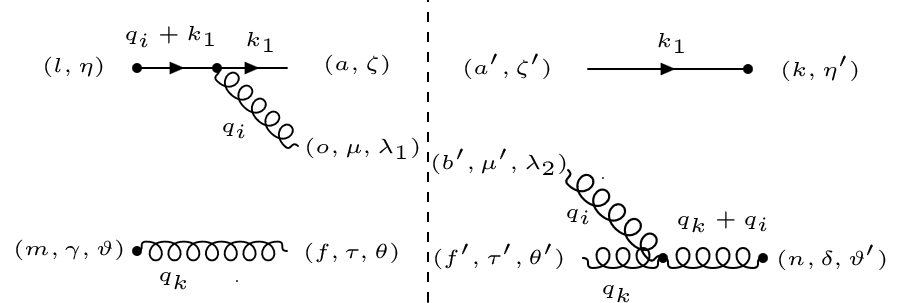
\includegraphics[scale=0.7]{images/GQ/M1M2DaggerGluonNew.png}
%\end{figure}
%
%\begin{equation}
%\begin{split}
%&M1{M_2}^{\dagger}=\frac{-{g_s}^2 {[T^{o}]_a}^{l} f^{\:f^{\prime}\: b^{\prime}\:n}}{4(k_1 \cdot q_i)(q_i \cdot q_k)}[\not{k_1}{\gamma}_{\mu}(\not{k_1}+\not{q_i})\:g^{\mu \mu^{\prime}}]\\
%&[ (g^{{{\tau}^{\prime}}{{\mu}^{\prime}}}(q_k-q_i)^{\delta}+g^{{{\mu}^{\prime}}{{\delta}}}(2q_i +q_k)^{{\tau}^{\prime}}-g^{\delta{{\tau}^{\prime}}}(2q_k+q_i)^{{\mu}^{\prime}})g^{\tau \tau^{\prime}}]\\
%\end{split}
%\end{equation}
%
%\begin{equation}
%\begin{split}
%&M1{M_2}^{\dagger}=\frac{-{g_s}^2 {[T^{o}]_a}^{l} f^{\:f^{\prime}\: b^{\prime}\:n}}{4(k_1 \cdot q_i)(q_i \cdot q_k)}[\not{k_1}{\gamma}_{\gamma}(\not{k_1}+\not{q_i})(q_k-q_i)^{\delta}+\not{k_1}{\gamma}^{\delta}(\not{k_1}+\not{q_i})(2q_i+q_k)_{\gamma}\\
%&-\not{k_1}(2\not{q_k}+\not{q_i})(\not{k_1}+\not{q_i}){g^{\delta}}_{\gamma}]\\
%\end{split}
%\end{equation}
%
%\begin{equation}
%\begin{split}
%&M1{M_2}^{\dagger}=\frac{-{g_s}^2 {[T^{o}]_a}^{l} f^{\:f^{\prime}\: b^{\prime}\:n}}{4(k_1 \cdot q_i)(q_i \cdot q_k)}[\not{k_1}(2\not{q_k}+\not{q_i})(\not{k_1}+\not{q_i})][-{g^{\delta}}_{\gamma}]\\
%\end{split}
%\end{equation}
%
%\begin{equation}
%\begin{split}
%&M1{M_2}^{\dagger}=\frac{-{g_s}^2 {[T^{o}]_a}^{l} f^{\:f^{\prime}\: b^{\prime}\:n}}{4(k_1 \cdot q_i)(q_i \cdot q_k)}
%[2\not{k_1}\not{q_k}\not{k_1}+2\not{k_1}\not{q_k}\not{q_i}+\not{k_1}\not{q_i}\not{k_1}+\not{k_1}\not{q_i}\not{q_i}][-{g^{\delta}}_{\gamma}]\\
%\end{split}
%\end{equation}
%
%\begin{equation}
%\begin{split}
%&M1{M_2}^{\dagger}=\frac{-{g_s}^2 {[T^{o}]_a}^{l} f^{\:f^{\prime}\: b^{\prime}\:n}}{4(k_1 \cdot q_i)(q_i \cdot q_k)}
%[4\not{k_1}(k_1 \cdot q_k)+2\not{k_1}\not{q_k}\not{q_i}+2\not{k_1}(k_1\cdot q_i)][-{g^{\delta}}_{\gamma}]\\
%\end{split}
%\end{equation}
%
%\begin{equation}
%\begin{split}
%&M1{M_2}^{\dagger}=\frac{-{g_s}^2 {[T^{o}]_a}^{l} f^{\:f^{\prime}\: b^{\prime}\:n}}{4(k_1 \cdot q_i)(q_i \cdot q_k)}
%\not{k_1}[4(k_1 \cdot q_k)+2\not{q_k}\not{q_i}+2(k_1\cdot q_i)][-{g^{\delta}}_{\gamma}]\\
%\end{split}
%\end{equation}
%
%\begin{equation}
%\begin{split}
%&M1{M_2}^{\dagger}=\frac{-{g_s}^2 {[T^{o}]_a}^{l} f^{\:f^{\prime}\: b^{\prime}\:n}}{4y\beta_1 (1-y)\:(p_i \cdot Q)(p_i \cdot p_k)}\\
%&((\alpha_1 -y\beta_1(\frac{Q^2}{2p_i \cdot Q})) \not{p_i} + y\beta_1\not{Q} + \sqrt{y\alpha_1\beta_1}\not{n}_{\bot,1} )\\
%&[4([\alpha_1 (1-y)+y\beta_1(\frac{Q^2}{2p_i \cdot Q})]\:p_i \cdot p_k+y\beta_1\:Q\cdot p_k+\sqrt{\alpha_1\beta_1y(1-y)} p_k \cdot {n_{\bot,1}})\\
%&+2(A_1\not{p_i} + A_2\not{Q} + \sqrt{1-y}\not{p_k})((\beta_1 -\alpha_1 y(\frac{Q^2}{2p_i \cdot Q}))\not{p_i} + y\alpha_1\not{Q} - \sqrt{y\alpha_1\beta_1}\not{n}_{\bot,1})\\
%&+2(y\:p_i\cdot Q)]\\
%&[-{g^{\delta}}_{\gamma}]\\
%\end{split}
%\end{equation}
%
%\begin{equation}
%\begin{split}
%&M1{M_2}^{\dagger}=\frac{-{g_s}^2 {[T^{o}]_a}^{l} f^{\:f^{\prime}\: b^{\prime}\:n}}{4y\beta_1 (1-y)\:(p_i \cdot Q)(p_i \cdot p_k)}\\
%&(1-\beta_1) \not{p_i} \\
%&[4(1-\beta_1) (1-y)\:p_i \cdot p_k\\
%&+2(A_1\not{p_i} + A_2\not{Q} + \sqrt{1-y}\not{p_k})((\beta_1 - y(\frac{Q^2}{2p_i \cdot Q}))\not{p_i} + y\not{Q} )\\
%&+2(y\:p_i\cdot Q)]\\
%&[-{g^{\delta}}_{\gamma}]\\
%\end{split}
%\end{equation}
%
%\begin{equation}
%\begin{split}
%&M1{M_2}^{\dagger}=\frac{-{g_s}^2 {[T^{o}]_a}^{l} f^{\:f^{\prime}\: b^{\prime}\:n}}{4y\beta_1 (1-y)\:(p_i \cdot Q)(p_i \cdot p_k)}\\
%&(1-\beta_1) \not{p_i} \\
%&[4(1-\beta_1) (1-y)\:p_i \cdot p_k\\
%&+2A_1y\not{p_i}\not{Q} + 2A_2(\beta_1 - y(\frac{Q^2}{2p_i \cdot Q}))\not{Q}\not{p_i}+2A_2yQ^2\\
%& + 2\sqrt{1-y}(\beta_1 - y(\frac{Q^2}{2p_i \cdot Q}))\not{p_k}\not{p_i}+ 2y\sqrt{1-y}\not{p_k}\not{Q}\\
%&+2y\:p_i\cdot Q]\\
%&[-{g^{\delta}}_{\gamma}]\\
%\end{split}
%\end{equation}
%
%\begin{equation}
%\begin{split}
%&M1{M_2}^{\dagger}=\frac{-{g_s}^2 {[T^{o}]_a}^{l} f^{\:f^{\prime}\: b^{\prime}\:n}}{4y\beta_1 (1-y)\:(p_i \cdot Q)(p_i \cdot p_k)}\\
%&[4(1-\beta_1)^2 (1-y)\:\not{p_i}\:\:(p_i \cdot p_k) + 4(1-\beta_1)\sqrt{1-y}(\beta_1 - y(\frac{Q^2}{2p_i \cdot Q}))\not{p_i\:\:}(p_k\cdot p_i)\\
%&+ 2(1-\beta_1)y\sqrt{1-y}\not{p_i}\not{p_k}\not{Q}+2y(1-\beta_1)\:\not{p_i}\:\:p_i\cdot Q][-{g^{\delta}}_{\gamma}]\\
%\end{split}
%\end{equation}
%
%\section{$ |M|^2 $}
%
%\begin{equation}
%\begin{split}
%&|M|^2=-d(1-\beta_1)\frac{{g_s}^2 C_F}{2y \:p_i \cdot Q}
%[  \not{p_i}][-{g^{\delta}}_{\gamma}]+2RE(\frac{-{g_s}^2 C_F}{4y\beta_1 (1-y)\:(p_i \cdot Q)(p_i \cdot p_k)}\\
%&[4(1-\beta_1)^2 (1-y)\:\not{p_i}\:\:(p_i \cdot p_k) + 4(1-\beta_1)\sqrt{1-y}(\beta_1 - y(\frac{Q^2}{2p_i \cdot Q}))\not{p_i\:\:}(p_k\cdot p_i)\\
%&+ 2(1-\beta_1)y\sqrt{1-y}\not{p_i}\not{p_k}\not{Q}+2y(1-\beta_1)\:\not{p_i}\:\:p_i\cdot Q][-{g^{\delta}}_{\gamma}])\\
%\end{split}
%\end{equation}
%
%\begin{equation}
%\begin{split}
%&|M|^2=-d(1-\beta_1)\frac{{g_s}^2 C_F}{2y \:p_i \cdot Q}
%[  \not{p_i}][-{g^{\delta}}_{\gamma}]+\frac{-{g_s}^2 C_F}{2y\beta_1 \:(p_i \cdot Q)}4(1-\beta_1)^2 (1-y)\:[\not{p_i}][-{g^{\delta}}_{\gamma}]\:\\
%&+\frac{-{g_s}^2 C_F}{2y\beta_1 (1-y)\:(p_i \cdot Q)} 4(1-\beta_1)\sqrt{1-y}(\beta_1 - y(\frac{Q^2}{2p_i \cdot Q}))[\not{p_i][-{g^{\delta}}_{\gamma}}]\\
%&+\frac{-{g_s}^2 C_F}{2y\beta_1 (1-y)\:(p_i \cdot Q)(p_i \cdot p_k)} 2(1-\beta_1)y\sqrt{1-y}\:[\not{p_i}\not{p_k}\not{Q}][-{g^{\delta}}_{\gamma}]\\
%&+\frac{-{g_s}^2 C_F}{4y\beta_1 (1-y)\:(p_i \cdot p_k)}2y(1-\beta_1)\:[\not{p_i}\:][-{g^{\delta}}_{\gamma}])\\
%\end{split}
%\end{equation}
%
%\begin{equation}
%\begin{split}
%&|M|^2=-(4-2\epsilon)(1-\beta_1)\frac{{g_s}^2 C_F}{2y \:(p_i \cdot Q)}
%[  \not{p_i}][-{g^{\delta}}_{\gamma}]+\frac{-{g_s}^2 C_F}{2y\beta_1 \:(p_i \cdot Q)}4(1-\beta_1)^2 (1-y)\:[\not{p_i}][-{g^{\delta}}_{\gamma}]\:\\
%&+\frac{-{g_s}^2 C_F}{2y\beta_1 (1-y)\:(p_i \cdot Q)} 4(1-\beta_1)\sqrt{1-y}(\beta_1 - y(\frac{Q^2}{2p_i \cdot Q}))[\not{p_i][-{g^{\delta}}_{\gamma}}]\\
%&+\frac{-{g_s}^2 C_F}{2y\beta_1 (1-y)\:(p_i \cdot Q)(p_i \cdot p_k)} 2(1-\beta_1)y\sqrt{1-y}\:[\not{p_i}\not{p_k}\not{Q}][-{g^{\delta}}_{\gamma}]\\
%&+\frac{-{g_s}^2 C_F}{4y\beta_1 (1-y)\:(p_i \cdot p_k)}2y(1-\beta_1)\:[\not{p_i}\:][-{g^{\delta}}_{\gamma}])\\
%\end{split}
%\end{equation}
%
%
%\begin{equation}
%\begin{split}
%&|M|^2=\frac{{g_s}^2 C_F}{2y \:(p_i \cdot Q)}
%[  \not{p_i}][{g^{\delta}}_{\gamma}][(4-2\epsilon)(1-\beta_1)+\frac{4(1-\beta_1)^2}{\beta_1}]
%\end{split}
%\end{equation}
%
%\begin{equation}
%\begin{split}
%&|M|^2=\frac{{g_s}^2 C_F}{2y \:(p_i \cdot Q)}
%[  \not{p_i}][{g^{\delta}}_{\gamma}][4-4\beta_1-2\epsilon +2\epsilon\beta_1+\frac{4(1-\beta_1)^2}{\beta_1}]
%\end{split}
%\end{equation}
%
%\begin{equation}
%	\left.\begin{aligned}
%\langle\:\hat{P_{qq}}\rangle &= C_F[\frac{1+z^2}{1-z}-\varepsilon(1-z)]\\
%\langle\:\hat{P_{gq}}\rangle &= T_R[1-\frac{2z(1-z)}{1-\varepsilon}]\\
%\langle\:\hat{P_{qg}}\rangle &= C_F[\frac{1+(1-z)^2}{z}-\varepsilon z]\\
%\langle\:\hat{P_{gg}}\rangle &= 2C_A[\frac{z}{1-z}+\frac{1-z}{z}+z(1-z)]
%\end{aligned}
%	\right\}
%	\quad \text{Alterali-Parisi
%	}
%\label{Alterali-Parisi}
%\end{equation}